\documentclass{article}
\usepackage[utf8]{inputenc}
\usepackage{graphicx}
\usepackage{amsmath}
\usepackage{amssymb}

\title{Intelligens Fejlesztőeszkozok - 4. órai jegyzet}
\author{Burian Sándor}
\date{Október 2022}

\begin{document}

\maketitle

\section{False Position metódus}

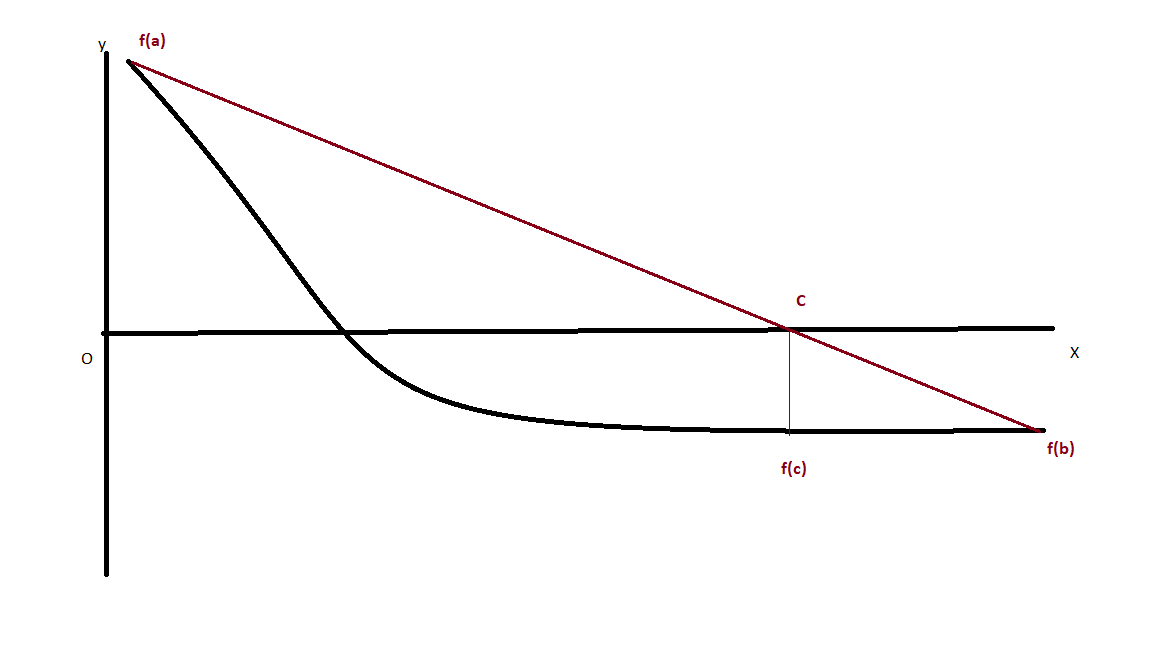
\includegraphics[scale=0.5]{../false_position.png} 

Intervallum felező + húr módszer:
\begin{itemize}
\item 1. húrt húzunk
\item 2. megkeressük a húr metszéspontját Ox tengelyen
\item 3. \textit{f(c) }és \textit{f(b)} előjele egyezik-e?
\item 4. \textit{f(c)} és \textit{f(a) }előjele egyezik-e?
\end{itemize}

Ekkor az f(a)f(c) szakasz az m1 es az f(c)f(b) az m2.

\begin{equation}
m = \dfrac{\Delta y}{\Delta x} \ 
\end{equation}

\begin{multline}
\\
\dfrac{f(b)-f(a)}{b-a} = \dfrac{c-f(b}{c-b}\\
\Rightarrow (c-b)(f(b)-f(a)) = (b-a)(-f(b)) \\
\Rightarrow (c-b) = -f(b) \dot{•} \dfrac{b-a}{f(b)-f(a)}\\
\\
\\
\Rightarrow c = b-f(b) \dot{•} \dfrac{b-a}{f(b)-f(a)}\\
\end{multline}

\section{Newton módszer}

\begin{equation}
x_{n+1} = x_n +\Delta x
\end{equation}

ahol:
\begin{itemize}
\item $x_n + \Delta x$ newtoni frissítés 
\item $\Delta x$ Newtoni lépés
\end{itemize}

\subsection{Newton-Raphson módszer}

\begin{equation}
\Delta x = \dfrac{f(x)}{f'(x)}
\end{equation}

Ekkor két eset lehetséges:
\begin{itemize}
\item létezik gyök $\Rightarrow $ konvergál
\item nem létezik gyök $\Rightarrow $ divergál
\end{itemize}

\begin{equation}
x_{n+1} = x- \gamma \Delta x  
\end{equation}

ahol $ \gamma \in (0,1]$

ha
\begin{itemize}
\item $\gamma < \Delta x $ akkor az kevesebb mint 1 lépés
\item $\gamma = \Delta x $ akkor az 1 lépés
\item $\gamma > \Delta x $ akkor viszalépek az utolsóra
\end{itemize}

\begin{equation}
f'( x_0 ) = \lim_{x \to x_0 } \dfrac{f(x)-f( x_0 )}{ x - x_0 }
\end{equation}

ahol $x = x_0 +h $

\begin{equation}
\dfrac{•}{•}
\end{equation}


\begin{equation}
\dfrac{f( x_0 +h) - f( x_0 )}{ x_0 + h - x_0 } = \dfrac{f( x_0 +h) - f( x_0 )}{h}
\end{equation}

\section{Kvázi Newton módszer}

általánosságban: $ x_{n+1} = x_n-\alpha_n \beta^{-1}_n \nabla f(x_n) $ ahol $\beta^{-1}_n $ a közelítő értéke a Hesse mátrixnak.

\subsection{Broydan módszere}

\begin{equation}
[f'( x_0 ) ]_{kozelitve} = \dfrac{f( x_k )- f( x_{k-1} )}{x_k - x_{k-1} } \Rightarrow x_{k+1} = x_k - \dfrac{f( x_k ) }{ [f'( x_k )]_{kozelitve} }
\end{equation}

$ \Rightarrow [f'( x_0 ) ]_{kozelitve} \dot{•} ( x_k - x_{k-1} ) = f( x_k ) - f( x_{k-1} ) \Rightarrow $

Általánosan: $ F(()): \mathbb{R} ^n \longrightarrow \mathbb{R}^n  J_k ( X_k - X_{k-1} ) = F( x_k )- F( x_{k-1} ) $ ahol $ J_k $ a jakobi mátrix.

\begin{multline}
\Delta X_k = X_k - X_{k-1} | \Delta F(k) = F( x_k) - F( x_{k-1} ) \Rightarrow J_k \Delta x_k = \Delta F( x_k ) \\
J_k = J_{k-1} + \dfrac{ \Delta F_k - J_{ k-1 } \Delta x_k }{ || \Delta x_2 ||^2 } \Delta x_2^T \\
\Rightarrow X_{n+1} = X_n - J_e^{-1} F( x_k )\\
\end{multline}

Euklédeszi norma: $ ||A||_F = \sqrt{  \sum_{i=1}^{m} \sum_{j=1}^{n} | a_{ij} |^2 } $

\section{Sherman - Morrison formula}

\begin{multline}
( A+uv^T )^{-1} = \dfrac{ A^{-1} uv^T A^{-1} }{ 1 + v^T A^{-1} u } \Rightarrow  \\
J_k^{-1} = J_{k-1}^{-1} + \dfrac{ \Delta x_k - J_{k-1}^{-1} \Delta F_k }{ \Delta x_k^T J_{k-1}^{-1} \Delta F_k }
\end{multline}

\subsection{Stephenson módszer}

Ha $ a $ kiindulási hely, $ b=g(a) $ és $ c = g(b) $ akkor 

\begin{equation}
\hat{p} = a \dfrac{ (b-a)^2 }{ a-2b+c }
\end{equation}

\end{document}
